\section{6 ottobre 2014}

\begin{enumerate}
    \item (1.20) Una persona ha 8 amici e decide di invitarne 5 a cena.
    \begin{itemize}
        \item In quanti modi pu\`o farlo se 2 amici non vanno d'accordo fra loro e non vogliono trovarsi insieme?
        \item In quanti modi pu\`o farlo se tra gli 8 amici c'\`e una coppia che non pu\`o essere divisa?
    \end{itemize}
    \item \label{esercizio_21} (1.21) Si consideri la griglia in figura \ref{fig:esercizio_21}. Si supponga di partire dal punto A spostandosi di volta in volta di un passo a destra o in alto, fino ad arrivare al punto B. Quanti sono i percorsi possibili? Si osservi che per raggiungere B da A si devono fare 4 passi a destra e 3 passi verso l'alto.
    \begin{figure}[ht]
    \centering
    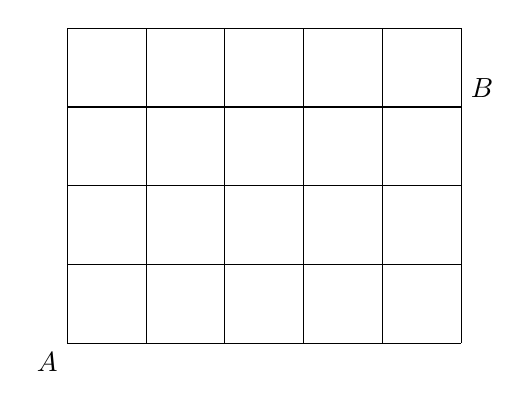
\begin{tikzpicture}
    \draw (0,0) grid (5,4);
    \draw (0,0) node[anchor=north east] {$A$};
    \draw (5,3) node[anchor=south west] {$B$};
    \end{tikzpicture}
    \caption{\label{fig:esercizio_21}Esercizio \ref{esercizio_21}}
    \end{figure}
    \item \label{esercizio_22} (1.22) Nel problema \ref{esercizio_21}, quanti sono i percorsi possibili che passano dal punto cerchiato in figura \ref{fig:esercizio_22}?
    \begin{figure}[ht]
    \centering
    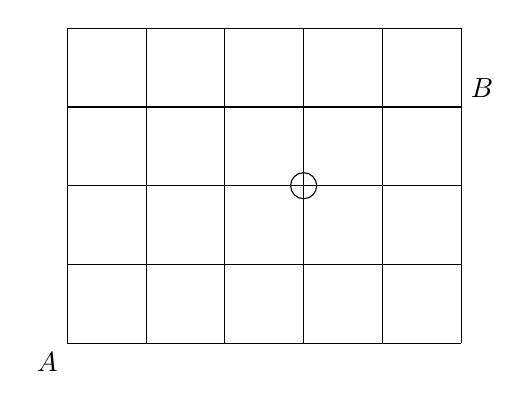
\begin{tikzpicture}
    \draw (0,0) grid (5,4);
    \draw (3,2) node[circle, draw] {};
    \draw (0,0) node[anchor=north east] {$A$};
    \draw (5,3) node[anchor=south west] {$B$};
    \end{tikzpicture}
    \caption{\label{fig:esercizio_22}Esercizio \ref{esercizio_22}}
    \end{figure}
    \item (1.23) Un laboratorio di psicologia che conduce degli esperimenti sui sogni dispone di 3 stanze con 2 letti ciascuna. In quanti modi si possono assegnare i letti a 3 coppie di gemelli in modo tale che ogni coppia di gemelli dorma nella stessa stanza?
    \item (1.27) In quanti modi si possono suddividere 12 persone in comitati di rispettivamente 3, 4 e 5 persone?
\end{enumerate}